Define the Hamiltonian in a second-quantized form and use this to compute the expectation value of the ground state (defining the so-called reference energy and later our Hartree-Fock functional) of
the helium atom.
Show that it is given by
\begin{equation}
    E[\Phi_0] = \expval{c}{\hat{H}}{c} = \sum_{i} \expval{i}{\hat{h}_0}{i} + \frac{1}{2} \sum_{ij} \left[\expval*{ij}{\frac{1}{r_{ij}}}{ij} - \expval*{ij}{\frac{1}{r_{ij}}}{ji}\right].
\end{equation}
Define properly the sums keeping in mind that the states $ij$ refer to all quantum numbers $n, l, m_l, s, m_s$.
Use the values for the various matrix elements listed at the end of the midterm to find the value of $E$ as function of $Z$ and compute $E$ as function of $Z$.

\subsection{}
We consider a Hamiltonian $\hat{H} = \hat{H}_0 + \hat{H}_I$, where $\hat{H}_0$ and $\hat{H}_I$ are one-electron and two-electron parts respectively, defined by
\begin{align}
    \hat{H}_0 &= \sum_{p q} \expval{p}{\hat{h}_0}{q} a_p^\dagger a_q, &
    \hat{H}_I &= \frac{1}{4} \sum_{pqrs} \expval{pq}{\hat{v}}{rs}_{AS} a_p^\dagger a_q^\dagger a_s a_r.
\end{align}

We have the normal-ordered form of annihilation and creation operators, relative to the reference state, where all creation operators are to the left of all annihilation operators.
For example, we have $N[a_p^\dagger a_q] = a_p^\dagger a_q$, $N[a_p a_q^\dagger] = -a_q^\dagger a_p$, where the sign is dependent on the number of permutations required to bring the operators to normal order.
We are interested in this, as
\begin{equation*}
    \expval{c}{N[A B\dotsm]}{c} = 0
\end{equation*}
if $N[A B \dotsm]$ is not empty, where $A, B, \dotsc$ are annihilation or creation operators.

With this, we have the contractions of operators, defined as
\begin{equation*}
    \wick{\c A \c B} = AB - N[AB].
\end{equation*}
Relative to our reference state, we have that
\begin{align*}
    \wick{\c a_i^\dagger \c a_j} &= \delta_{i j}, &
    \wick{\c a_a \c a_b^\dagger} &= \delta_{a b}
\end{align*}
are the only non-zero contractions.

For the one-body term, we then have
\begin{equation}
    \expval{c}{\hat{H}_0}{c} = \sum_{pq} \expval{p}{\hat{h}_0}{q} \expval{c}{a_p^\dagger a_q}{c} = \sum_{ij} \expval{i}{\hat{h}_0}{j} \delta_{ij} = \sum_{i} \expval{i}{\hat{h}_0}{i}.
\end{equation}

For the two-body term, writing $\ket{c} = \ket{i j}$ we first need to examine the possible contractions of $ i j p^\dagger q^\dagger s r j^\dagger i^\dagger$ and the resulting matrix element $\expval{pq}{V}{rs}_{AS}$.
We have
\begin{align*}
    \wick{
        \c2 j
        \c1 i
        \c1 p^\dagger
        \c2 q^\dagger
        \c2 s
        \c1 r
        \c1 i^\dagger
        \c2 j^\dagger
    } &= \delta_{jq} \delta_{ip} \delta_{sj} \delta_{ri} \to \expval{ij}{V}{ij}_{AS}, \\
    \wick{
        \c2 j
        \c1 i
        \c1 p^\dagger
        \c2 q^\dagger
        \c2 s
        \c1 r
        \c2 i^\dagger
        \c1 j^\dagger
    } &= -\delta_{jq} \delta_{ip} \delta_{si} \delta_{rj} \to -\expval{ij}{V}{ji}_{AS}, \\
    \wick{
        \c2 j
        \c1 i
        \c2 p^\dagger
        \c1 q^\dagger
        \c2 s
        \c1 r
        \c2 i^\dagger
        \c1 j^\dagger
    } &= \delta_{jp} \delta_{iq} \delta_{si} \delta_{rj} \to \expval{ji}{V}{ji}_{AS}, \\
    \wick{
        \c2 j
        \c1 i
        \c2 p^\dagger
        \c1 q^\dagger
        \c2 s
        \c1 r
        \c1 i^\dagger
        \c2 j^\dagger
    } &= -\delta_{jp} \delta_{iq} \delta_{sj} \delta_{ri} \to -\expval{ji}{V}{ij}_{AS}.
\end{align*}
As $\expval{\alpha \beta}{V}{\gamma \delta}_{AS} = - \expval{\alpha \alpha}{V}{\delta \gamma}_{AS}$ we gather these terms, and inserting for $V$, leaving us with
\begin{equation}
    \expval{c}{\hat{H}_I}{c} = \frac{1}{2} \sum_{ij} \expval{ij}{\frac{1}{r_{ij}}}{ij}_{AS} = \frac{1}{2} \sum_{ij} \expval{ij}{\frac{1}{r_{ij}}}{ij} - \expval{ij}{\frac{1}{r_{ij}}}{ji}.
\end{equation}

Combining this with the one-body term, we have the total reference energy
\begin{equation}
    E[\Phi_0] = \expval{c}{\hat{H}}{c} = \sum_{i} \expval{i}{\hat{h}_0}{i} + \frac{1}{2} \sum_{ij} \expval{ij}{\frac{1}{r_{ij}}}{ij} - \expval{ij}{\frac{1}{r_{ij}}}{ji},
\end{equation}
as we wanted to show.

In the case of the electrons in the helium atom, we only have $n = 1$, $l = 0$, differing only in the spin quantum number $m_s = \pm 1/2$.
The expectation value of the one-body part is then
\begin{equation*}
    \expval{\Phi_0}{\hat{H}_0}{\Phi_0} = \sum_{\sigma \in \{\pm 1/2\}} \expval{1\sigma}{\hat{h}_0}{1\sigma} = -Z^2,
\end{equation*}
and the expectation value of the two-body part is, writing just $\sigma_{+}$ and $\sigma_{-}$ for the spins with $n = 1$,
\begin{equation*}
    \expval{\Phi_0}{\hat{H}_I}{\Phi_0}
    = \frac{1}{2} \sum_{\substack{\sigma_{+}\sigma_{-}\\ \sigma_{+} \neq \sigma_{-}}}
    \underbrace{\expval*{\sigma_{+} \sigma_{-}}{\frac{1}{r_{\sigma_{+}\sigma_{-}}}}{\sigma_{+} \sigma_{-}}}_{\textnormal{Direct term}}
    - \underbrace{\expval*{\sigma_{+} \sigma_{-}}{\frac{1}{r_{\sigma_{+}\sigma_{-}}}}{\sigma_{-}\sigma_{+}}}_{\textnormal{Exchange term}}.
\end{equation*}
The exchange term vanishes since the states are orthogonal, and we are left with the direct term.
We are then just left with
\begin{equation*}
    \expval{\Phi_0}{\hat{H}_I}{\Phi_0} = \frac{1}{2}\left[ \expval*{\sigma_{+} \sigma_{-}}{\frac{1}{r_{\sigma_{+} \sigma_{-}}}}{\sigma_{+} \sigma_{-}} + \expval*{\sigma_{-} \sigma_{+}}{\frac{1}{r_{\sigma_{+} \sigma_{-}}}}{\sigma_{-} \sigma_{+}}\right].
\end{equation*}
As $\hat{H}_I$ is invariant under the change of label $\sigma$, we can simplify this to
\begin{equation*}
    \expval{\Phi_0}{\hat{H}_I}{\Phi_0} = \expval*{\sigma_{+} \sigma_{-}}{\frac{1}{r_{\sigma_{+} \sigma_{-}}}}{\sigma_{+} \sigma_{-}} = \frac{5}{8} Z.
\end{equation*}

Combining this, we find that the expectation value of the ground state is
\begin{equation}
    E[\Phi_0] = -Z^2 + \tfrac{5}{8}Z,
\end{equation}
which as a function of $Z$ is shown in \autoref{fig:energy}.

\begin{figure}[ht]
    \centering
    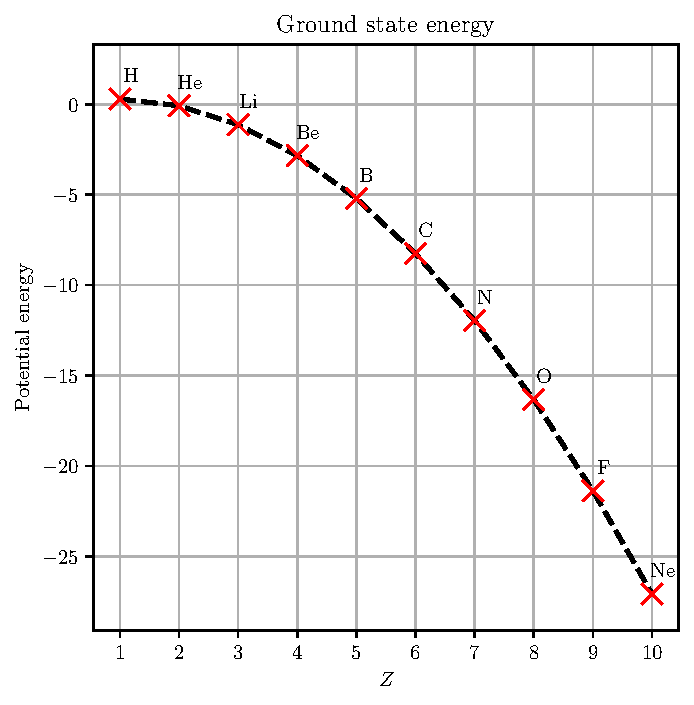
\includegraphics{figs/energy_plot.pdf}
    \caption{The expectation value of the ground states of an atom with two electrons as a function of the nuclear charge $Z$.\label{fig:energy}}
\end{figure}
